\addtocontents{toc}{\protect\setcounter{tocdepth}{1}}
\chapter*{APÊNDICE B - DOCUMENTO DE REQUISITOS}\label{apendice_requisitos}
\addcontentsline{toc}{chapter}{APÊNDICE B - DOCUMENTO DE REQUISITOS}
\addtocontents{toc}{\protect\setcounter{tocdepth}{-1}}


\section{Introdução}
Este documento especifica os requisitos do sistema AskMath, fornecendo aos desenvolvedores as informações necessárias para o projeto e implementação, assim como para a realização dos testes. 

\subsection{Visão geral do documento}
O documento apresenta os requisitos funcionais, onde para cada um destes define seu caso de uso e sua descrição detalhada. Além disso, define sua prioridade, explicado no tópico abaixo, e suas pré e pós condições, entradas e saídas caso existam. Logo em seguida, será apresentado os diagramas de caso de uso do sistema e alguns caso de usos críticos, e por fim o grafo de rastreabilidade entre os requisitos.

\subsection{Prioridades dos requisitos}
Cada requisito terá uma determinada prioridade, essa prioridade ira ajudar a equipe de desenvolvimento na escolha de quais requisitos mais se preocupar quando tiver desenvolvendo o sistema, criamos para isso, três níveis prioridades:

\begin{alineascomponto}
	\item Essencial: requisito é o requisito ao qual o sistema não entra em funcionamento sem ele. Esses requisitos tem que ser implementados o mais rápido possível. 
    \item Importante: requisito sem o qual o sistema entra em funcionamento, mas de forma não satisfatória. Esse requisitos deverão sem implementados, mas caso não sejam, o sistema ainda poderá funcionar consideravelmente.
	\item Desejável: requisito que não compromete o sistema, esse tipo de requisito é comumente deixado para versões posteriores do sistema.
\end{alineascomponto}

\section{Requisitos Funcionais}

\fbox{
\parbox{\textwidth}{
  \begin{center}
  [RF001] Tipos de Usuário e Autenticação
  \end{center}
O Sistema deverá possuir quatro tipos de Estudantes, Bolsistas, Professores e Administradores, e todos deverão ser autenticados; para isso, o mesmo deverá possuir um procedimento de autorização de utilizadores, onde cada utilizador se deve identificar através de um nome de usuário e uma senha. Apenas os utilizadores autorizados dessa forma podem acessar o sistema.
\linebreak
Prioridade: Essencial
}}


\fbox{
\parbox{\textwidth}{
  \begin{center}
  [RF002] Cadastro
  \end{center}
Alunos podem se cadastrar no sistema. Quando o usuário não possuir nenhum código especial para se cadastrar, a única opção disponível para ele sera de Aluno.
\linebreak
Prioridade: Essencial
}}


\fbox{
\parbox{\textwidth}{
  \begin{center}
  [RF003] Recuperar Senha
  \end{center}
O Sistema deverá propiciar aos usuário uma opção para recuperar sua senha caso necessite.
\linebreak
Prioridade: Essencial
}}


\fbox{
\parbox{\textwidth}{
  \begin{center}
	[RF004] Hierarquia do Conteúdos
  \end{center}
No sistema, existem disciplinas, lições para as disciplinas e problemas para as 
lições. Os professores poderão cadastrar várias disciplinas, e para cada 
disciplina, poderá ser cadastradas várias lições. Quando o Aluno entrar no 
sistema, ele poderá ver apenas as lições de uma determinada disciplina por vez, 
podendo alternar entre disciplinas. Os bolsistas irão adicionar problemas as 
lições, sendo assim, para poder um aluno responder uma lição, ele terá de 
escolher uma disciplina, depois uma lição e por fim a problema.
\linebreak
Prioridade: Essencial
}}


\fbox{
\parbox{\textwidth}{
  \begin{center}
	[RF007] Estrutura do Problema
  \end{center}
Cada problema poderá possuir vários itens. Os problema serão somente de 
múltipla escolha, ele poderá possuir no mínimo dois itens e no máximo cinco 
itens, essa quantidade fica a critério do bolsista que a está cadastrado no 
sistema.
\linebreak
Prioridade: Essencial
}}

\fbox{
\parbox{\textwidth}{
  \begin{center}
	[RF008] Manter Disciplinas
  \end{center}

Professores poderão adicionar, editar e excluir disciplinas e lições.
\linebreak
Prioridade: Essencial
}}

\fbox{
\parbox{\textwidth}{
  \begin{center}
	[RF009] Manter Problemas
  \end{center}
Assistentes poderão adicionar, editar e excluir problemas das lições.
\linebreak
Prioridade: Essencial
}}

\fbox{
\parbox{\textwidth}{
  \begin{center}
	[RF0010]Alternar entre Disciplinas
  \end{center}
Quando o aluno entrar no sistema pela primeira vez, ele verá uma lista com as 
disciplinas disponíveis, ele então deverá escolher uma opção, em seguida irão 
aparecer apenas lições referentes aquela disciplina, mas caso ele queira, ele 
poderá trocar facilmente de disciplina.
\linebreak
Prioridade: Essencial
}}

\fbox{
\parbox{\textwidth}{
  \begin{center}
	[RF0011] Ver Detalhes da Lição
  \end{center}
Antes de começar a resolver os problemas de determinada lição, o aluno deverá 
ver informações daquela lição.
\linebreak
Prioridade: Essencial
}}

\fbox{
\parbox{\textwidth}{
  \begin{center}
	[RF0012] Sair da Lição
  \end{center}
O Aluno poderá sair da lição antes mesmo de tê lá concluído, voltando depois da 
posição onde parrou. Ao sair, o aluno deverá ver estatísticas referentes a 
evolução dele na lição.
\linebreak
Prioridade: Essencial
}}

\fbox{
\parbox{\textwidth}{
  \begin{center}
	[RF0012] Saltar Problemas
  \end{center}
O sistema deverá permitir ao aluno, saltar problemas e rever os saltos 
realizados, isso com algumas restrições de quantidade de vezes.
\linebreak
Prioridade: Essencial
}}

\fbox{
\parbox{\textwidth}{
  \begin{center}
	[RF0013] Pedir ajuda
  \end{center}
Para todo problema, o sistema dever\'a apresentar um bot\~ao de ajuda. Ao 
clique do Aluno, o sistema dever\'a perguntar ao aluno se ele deseja obter 
ajuda do sistema ou de algu\'em que j\'a concluiu aquela li\c{c}\~ao com bom 
aproveitamento. Caso o aluno opte pela primeira op\c{c}\~ao, o sistema 
exibir\'a um texto de ajuda cadastrado pelo assistente durante a cria\c{c}\~ao 
do problema. J\'a no caso dele escolher a segunda op\c{c}\~ao, o sistema ir\'a 
notificar aos alunos que estiverem online no momento que j\'a concluirão aquela 
li\c{c}\~ao com certa pr\'o-efici\^encia e caso algum deles aceite o pedido de 
ajuda, os dois encontram numa sala de bata-papo para conversar.  
\linebreak
Prioridade: Essencial
}}

\fbox{
\parbox{\textwidth}{
  \begin{center}
	[RF0014]  Alterar Visibilidade do Problema
  \end{center}
Um problema pode ser visível aos alunos ou não, quando o assistente estiver 
adicionando um problema, terá um campo mancado por padrão como verdadeiro que 
indicará se o problema estará visível ou não para os alunos, caso o mesmo não 
queira que o problema adicionado fique imediatamente visível aos alunos, ele 
desmarcar\'a esse campo e futuramente ele poderá editar o problema e marca-lo 
quando quiser que os alunos possam acessá-la.
\linebreak
Prioridade: Essencial
}}

\fbox{
\parbox{\textwidth}{
  \begin{center}
	[RF0015] Deficiências
  \end{center}
Cada item incorreto de um problema, deverá linkar para uma deficiência, essa 
deficiência é outra lição. Pode ser possível, a partir de um item respondido 
incorretamente em um problema, identificar a deficiência do aluno, por isso, é 
fundamental que no momento que o assistente estiver adicionando os itens do 
problema, ele poder\'a escolher para os itens incorretos, uma ou várias outras 
lições, essas lições ficarão sendo as supostas deficiências do aluno caso ele 
erre aquele problema respondendo aquele item.
\linebreak
Prioridade: Essencial
}}

\fbox{
\parbox{\textwidth}{
  \begin{center}
	[RF0016] Recompensas e Punições
  \end{center}
A cada 3 problemas que o aluno responder corretamente, ele será parabenizado e 
ganhará um prêmio e a cada 3 errados ele será penalizado. Quando o aluno 
resolver seguidamente três problemas corretamente, os seus pontos acumulados 
irão dobrar e a cada vez que ele errar três questões seguidamente, seus pontos 
acumulados serão subtraídos em 25%.
\linebreak
Prioridade: Essencial
}}

\fbox{
\parbox{\textwidth}{
  \begin{center}
	[RF0017] Fórum
  \end{center}
Caso o aluno possua alguma dúvida, o sistema deverá possuir um fórum onde esse 
aluno poderá postar suas dúvidas, para que professores, bolsistas ou outros 
alunos possam lhes ajudar com o problema, nesse fórum, deve possuir tópicos, 
comentários para os tópicos e nos comentários devem oferecer uma opção para ele 
comentar com imagem.
\linebreak
Prioridade: Essencial
}}

\fbox{
\parbox{\textwidth}{
  \begin{center}
	[RF0018] Ordenar Problemas
  \end{center}
O Sistema deve apresentar ao bolsista uma forma simples para ele ordenar a 
sequência dos problemas de cada lição.
\linebreak
Prioridade: Essencial
}}

\fbox{
\parbox{\textwidth}{
  \begin{center}
	[RF0018] Suporte a Latex
  \end{center}
O Sistema deve permitir ao bolsista adicionar código Latex(funções) na criação 
dos problemas e lições. Quando os bolsista adicionarem os problemas, o sistema 
devera reconhecer código Latex referente a fórmulas matemáticas. Toda vez que o 
bolsista colocar um código Latex entre as tgs '\$', o sistema deverá reconhecer 
isso, e mostrar para o usuário a imagem da fórmula referente aquele código.
\linebreak
Prioridade: Essencial
}}


\section{Requisitos N\~ao Funcionais}

\fbox{
\parbox{\textwidth}{
  \begin{center}
	[RN001] Tecnologias
  \end{center}
O Sistema deve ser desenvolvido apenas com tecnologias open source.
\linebreak
Prioridade: Essencial
}}

\fbox{
\parbox{\textwidth}{
  \begin{center}
	[RN002] Persistência dos Dados
  \end{center}
O sistema deverá utilizar como sistema de gerenciamento de banco de dados o 
PostgresSQL.
\linebreak
Prioridade: Importante
}}

\fbox{
\parbox{\textwidth}{
  \begin{center}
	[RN003] Segurança
  \end{center}
O sistema não apresentará aos usuários quaisquer dados de cunho privativo.
\linebreak
Prioridade: Essencial
}}

\fbox{
\parbox{\textwidth}{
  \begin{center}
	[RN004] Estrutura
  \end{center}
O sistema deverá ser desenvolvido de forma modularizada, para permitir a 
reusabilidade de tais módulos por outras aplicações no futuro. 
\linebreak
Prioridade: Essencial
}}

\fbox{
\parbox{\textwidth}{
  \begin{center}
	[RN005] Padrões
  \end{center}
O Sistema deverá ser desenvolvido utilizando os princípios de Orientação a 
Objetos.
\linebreak
Prioridade: Essencial
}}

\fbox{
\parbox{\textwidth}{
  \begin{center}
	[RN006] Ambiente de Execução
  \end{center}
O sistema deverá ser acessado completamente via browser HTTP/HTML. 
\linebreak
Prioridade: Essencial
}}

\fbox{
\parbox{\textwidth}{
  \begin{center}
	[RN007] Acessibilidade
  \end{center}
O Sistema devera possuir Responsive Web Design, assim como as v\'arias 
diretivas de acessibilidade para web.
\linebreak
Prioridade: Importante
}}

\fbox{
\parbox{\textwidth}{
  \begin{center}
	[RN008] Internacionalização
  \end{center}
O Sistema será disponibilizado em inglês, mas de forma a permitir que versões em 
línguas latinas possam ser produzidas sem necessidade de ter acesso ao código 
fonte.
\linebreak
Prioridade: Importante
}}

\fbox{
\parbox{\textwidth}{
  \begin{center}
	[RN009] Desempenho
  \end{center}
Quando um aluno responder um problema, a correção devera ser apresentada ao 
aluno, no máximo, em 2 segundos.
\linebreak
Prioridade: Essencial
}}

\fbox{
\parbox{\textwidth}{
  \begin{center}
	[RN010] Log do Sistema
  \end{center}
O Sistema devera salvar um histórico de todas as ações que os usuários 
realizarem.
\linebreak
Prioridade: Essencial
}}


\fbox{
\parbox{\textwidth}{
  \begin{center}
	[RN010] Log do Sistema
  \end{center}
O Sistema devera salvar um histórico de todas as ações que os usuários 
realizarem.
\linebreak
Prioridade: Essencial
}}

\section{Requisitos de Domínio}

\fbox{
\parbox{\textwidth}{
  \begin{center}
	[RN001] Log do Sistema
  \end{center}
O Sistema devera salvar um histórico de todas as ações que os usuários 
realizarem.
\linebreak
Prioridade: Essencial
}}

\section{Casos de uso}

\begin{figure}[H]
\centering
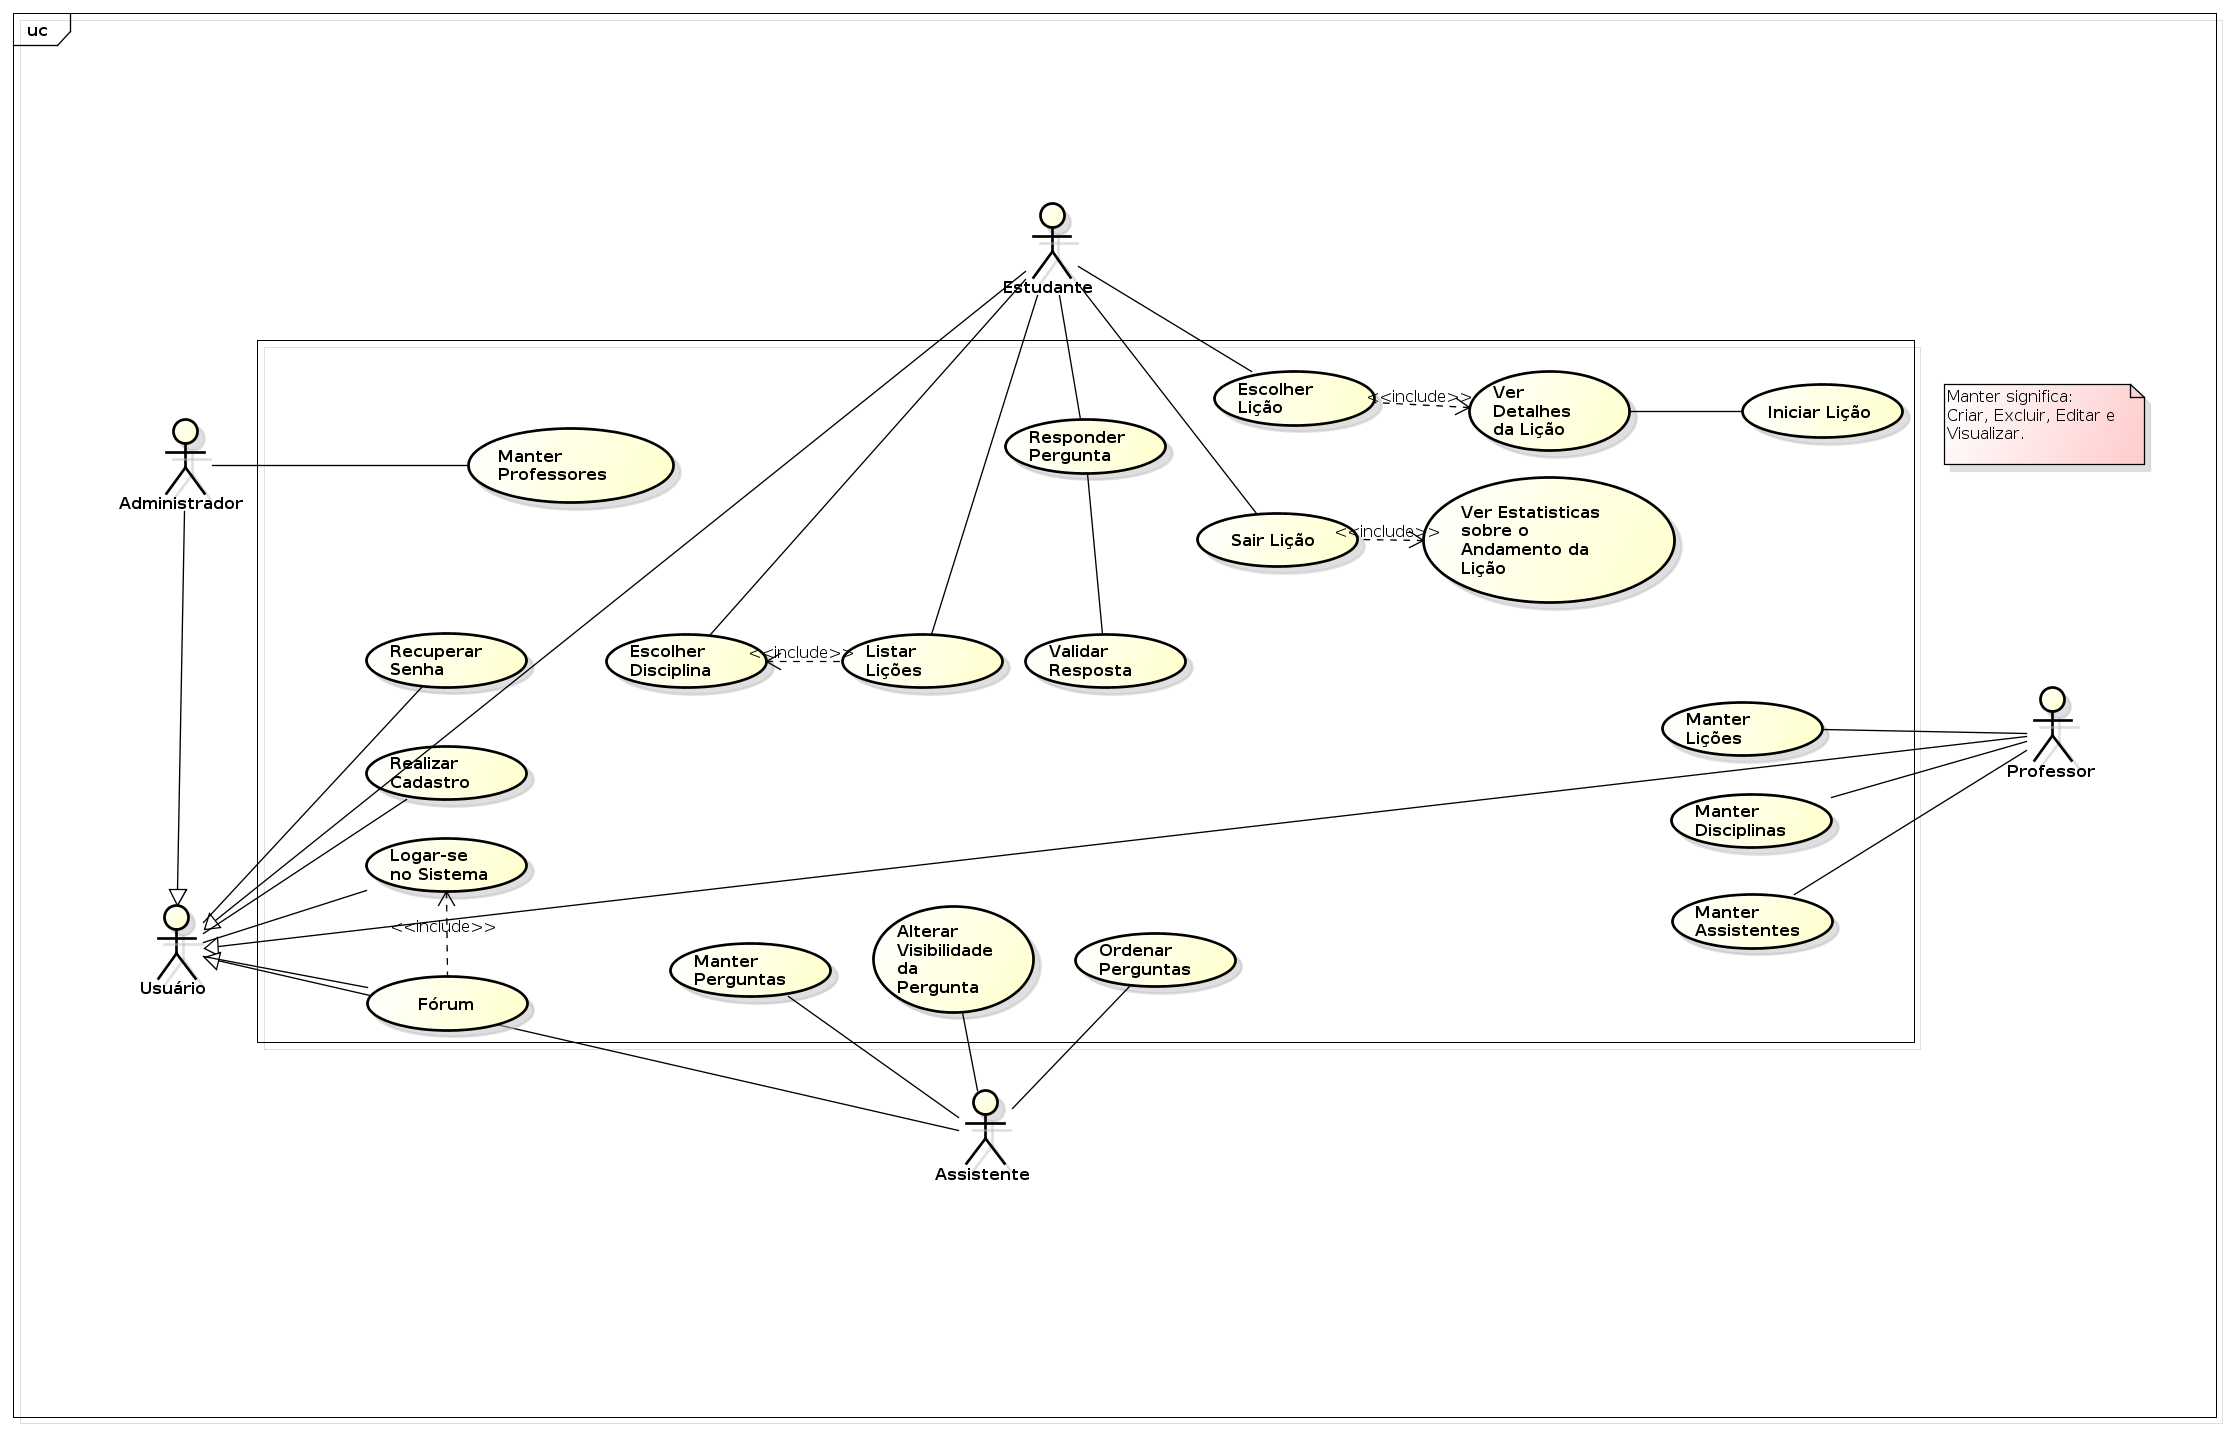
\includegraphics[width=18cm]{figuras/figura_casos_de_uso}
\caption{Diagrama de Casos de Uso}
\label{figura_casos_de_uso}
\end{figure}

\subsection{Descri\c{c}\~ao dos Casos de Uso}

\begin{alineascomponto}
	\item Manter Professor: O Administrador terá uma opção onde poderá manter 
professores: isso funcionara da seguinte forma: Para cadastrar, o Administrador 
logado, gera um código de alguns caracteres e dar ao professor, o professor de 
posse desse código, entra na tela de cadastro dos usuário e escolhe o tipo de 
usuário que ele quer se cadastrar e informa o código de acesso que ele possui, 
assim ele terá permissão para se cadastrar como Professor.

	\item Manter Assistente: De forma análoga ao Administrador, o professor 
também irá gerar um código e entregar ao assistente, o assistente de posse 
desse código irá entrar na tela de cadastro do sistema, informar o tipo de 
usuário e o código de acesso.

	\item Recuperação de Senha: No momento do cadastro, cada usuário devera 
indicar um email v\'alido, caso futuramente o usuário necessite 
alterar a senha, um email será enviado à esse email cadastrado com um link onde 
o mesmo poder\'a acessar para recuperar a senha.

	\item Manter Conte\'udos: Apenas os professores terão permissão para manter 
conte\'udos e lições, ao adicionar uma lição, ele terá que informar apenas o 
nome da lição e ao adicionar uma lição, ele terá que informar os 
Pré-Requisitos(Outras lições que eles recomendam ter sido concluídas para se 
prosseguir na atual) e Sugestões de Estudo (outras lições que eles recomendam 
seguir após concluir essa lição) para aquela lição assim como a quantidade 
máxima de pulos que o aluno poderá realizar naquela lição.

	\item Manter Problemas: Cada lição possuirá uma lista de problemas e os 
mesmos serão adicionadas pelos assistentes. Quando um assistente adicionar 
um problema, ele terá de informar a qual lição que ele pertence, os itens que 
ela terá, assim como o item correto, a ajuda caso esse problema necessite ter, 
a quantidade de pontos que ele terá e se ele irá ficar visível imediatamente 
para os alunos ou não.

	\item Ver Detalhes da Lição: Quando o aluno optar por responder as perguntas 
de uma determinada lição, antes de mais nada, ele precisa saber os detalhes 
daquela lição, detalhes do tipo: Quantidade de questões, Máximo de Saltos 
Permitidos, Pré-Requisitos, Curiosidades sobre o conteúdo daquela lição.

	\item Sair da Lição: Enquanto o aluno estiver resolvendo os problemas, o 
sistema devera lhe oferecer a opção dele sair da lição, quando ele sair, ele 
terá de ver as estatísticas referentes ao andamento dele naquela lição como: 
Acertos, Erros, Saltos, Quantidade de Pontos Acumulados e também uma lista com 
as lições sugeridas.
	
	\item Ordenar Problemas: Quando o bolsista adicionar um problema, ela será 
adicionada automaticamente logo depois dos outros problemas daquela lição(se 
pensarmos numa lista), mas ele deverá ter uma opção onde apenas arrastando 
os problema de posição ele possa reordena-los, utilizando apenas o mouse.

\end{alineascomponto}